\documentclass[12pt]{report}
\usepackage{setspace}
\usepackage{titlesec}
\usepackage[utf8]{inputenc}
\usepackage[top=1in,bottom=1in,left=1.5in,right=1in,headheight=0.5in,headsep=0.5in]{geometry}
\usepackage{graphicx}
\usepackage{subcaption}
\usepackage{amsmath,amssymb,amsfonts}
\usepackage[hidelinks]{hyperref}
\usepackage{cite}
\usepackage{float}
\usepackage{array}
\usepackage{caption}
\usepackage{multirow}
\usepackage[table]{xcolor}
\usepackage{fix-cm} % Allow arbitrary scaling of fonts

% custom command for chapter headings
\titleformat{\chapter}[display]
  {\rmfamily\bfseries\fontsize{16}{18}\selectfont}{\chaptertitlename\ \thechapter}{20pt}{\fontsize{16}{18}\selectfont\bfseries}

% setting for section headings
\titleformat{\section}[block]
  {\rmfamily\bfseries\fontsize{14}{16}\selectfont}{\thesection}{1em}{}

% setting for subsection headings
\titleformat{\subsection}[block]
  {\rmfamily\bfseries\fontsize{13}{14}\selectfont}{\thesubsection}{1em}{}

% setting for subsubsection headings
\titleformat{\subsubsection}[block]
  {\rmfamily\bfseries\fontsize{12}{12}\selectfont}{\thesubsubsection}{1em}{}



% adjusting spacing before and after paragraphs
\setlength{\parindent}{0pt}
\setlength{\parskip}{6pt}

% adjusting line spacing
\onehalfspacing

\begin{document}
      \begin{center}
		\thispagestyle{empty}
		\Large\textbf{TRIBHUVAN UNIVERSITY}\\
		\Large\textbf{INSTITUTE OF ENGINEERING }\\
		\vspace{0.2in}
		\large{\textbf{Khwopa College Of Engineering}\\}
		\normalsize{Libali, Bhaktapur\\}
		\large\textbf{Department of Computer Engineering}
		\vspace{0.2in}
		\begin{figure}[h]
		    \centering
			    
\includegraphics{img/Khwopalogo.jpg}
		\end{figure}
		
		\vspace{0.2in}
		\large{A PROPOSAL ON\\\textbf{DEEPFAKE IMAGE  DETECTION USING ResNet ARCHITECTURE}\\}
	
		\vspace{0.2in}
		\large{\textit{Submitted in partial fulfillment of the requirements for the degree\\}}
		
		\vspace{0.2in}
		\large{\textbf{BACHELOR OF COMPUTER ENGINEERING}\\}
		
		\vspace{0.2in}
		\large{Submitted by}\\
		\vspace{0.1in}
		\begin{tabular}{p{3.5in}p{2in}}
			\hspace{0.3cm}Manish Pyakurel& \hspace{1cm}KCE077BCT020\\
			\hspace{0.3cm}Rupak Neupane& \hspace{1cm}KCE077BCT028\\
			\hspace{0.3cm}Sarjyant Shrestha& \hspace{1cm}KCE077BCT033\\
			\hspace{0.3cm}Srijan Gyawali& \hspace{1cm}KCE077BCT036\\
		\end{tabular}
		\\
		\vspace{1cm}
		% \large{\textbf{Under the Supervision of}\\}
		% 	\normalsize{Er.Dinesh Gothe\\
		% 		Department Of Computer Engineering\\
		% 	}
			\vspace{0.8cm}
		\large{\textbf{Khwopa College Of Engineering}\\}
			\normalsize{Libali, Bhaktapur\\
			2023
		}
    \end{center}

       \chapter{Introduction}
        \pagenumbering{arabic}
        \section{Background Introduction}
        In recent years, the landscape of digital image manipulation has undergone a transformative shift with the emergence of deep fake techniques. This innovative approach, rooted in deep learning methodologies, has gained significant traction as a means of fabricating images by seamlessly replacing facial features from one individual with those of another. Coined as "deep fakes" by a Reddit user in 2017, these manipulations often leverage advanced adversarial models, such as Generative Adversarial Networks (GANs). Notably, this technology has been controversially utilized to superimpose celebrity faces onto explicit content, raising concerns related to fake pornography, misinformation, financial fraud, and hoaxes.
        Despite the ethical challenges associated with deep fakes, it is essential to acknowledge the positive applications within fields such as virtual reality, film editing, and production. The core working principles behind deep fakes involve intricate processes of merging, replacing, combining, and superimposing images. Leveraging deep learning and machine learning techniques, these manipulations give rise to convincingly altered digital images and videos, demonstrating both the potential benefits and ethical considerations associated with this rapidly advancing technology.
        \section{Problem Statement}
        In the rapidly evolving landscape of computer and automation technologies, the realm of possibilities continues to expand. Artificial Intelligence (AI) stands as a pivotal force, driving unprecedented advancements in areas such as predictive analytics, weather forecasting, automation, and the creation of sophisticated entities like deep fakes, which encompass AI-generated videos, audios, and images. While these technological strides are undeniably transformative, the misuse and exploitation of such capabilities pose significant concerns. 

        In recent times, there's been a surge in the creation of deep fakes, where the faces of celebrities or ordinary people are manipulated using just a single image and advanced deep learning algorithms. This issue is becoming more significant, as it circulates potentially harmful and illegal images of the victims to the public.

        The rise of these deceptive practices not only threatens individual privacy but also has broader implications for public trust and safety. As deep fakes become increasingly convincing, the potential for malicious use, misinformation, and damage to reputations grows. It is crucial to address this issue head-on by developing sophisticated detection mechanisms to safeguard against the harmful consequences of manipulated images. This proposal seeks to contribute to the ongoing efforts in mitigating the risks associated with deep fakes, reinforcing the integrity of visual content in the age of advanced AI technologies.
       \section{Obejctive}
            The main aim of this project is:
            \begin{itemize}
                \item To identify manipulated digital media content, particularly facial features and images.
                \item To implement cutting-edge deep learning and machine learning techniques.
            \end{itemize}
  \chapter{Literature Review}
Deepfakes, which involve the unauthorized swapping of face images, are frequently carried out without the knowledge or consent of individuals, including celebrities and politicians. Notably, historical instances, such as the facial image swapping in a photograph of Abraham Lincoln (Badale et al., 2018), underscore the longstanding nature of this challenge. Addressing these concerns, Yang, Li \& Lyu (2019) proposed a model leveraging head pose inconsistency to detect deepfakes, enabling the creation of synthetic faces for various individuals while preserving the original facial expressions.
Jagdale \& Shah (2019) introduced the NA-VSR algorithm for super resolution, involving video conversion into frames, median filtering to remove noise, and bicubic interpolation for pixel density enhancement. Additionally, Yadav \& Salmani (2019) elucidated the working principles of deep fake techniques, emphasizing the high precision value in face image swapping.
Generative Adversarial Neural Networks (GANs) play a pivotal role in deepfake generation, comprising a generator and a discriminator. The generator synthesizes fake images from a given dataset, while the discriminator evaluates the authenticity of the generated images. The inherent risks of deepfakes, including character defamation, potential harm to individuals, and the dissemination of fake news in society, highlight the importance of addressing these challenges.
Existing approaches encounter issues such as inefficiency in detecting deepfake images, high error rates, prolonged computation times, and data access inaccuracies. Our work focuses on improving the efficiency by using a different approach of using ResNet150 architecture for deepfake detection.Figure 1 presents a compilation of related works for deepfake detection (Heidari et al., 2022).

\begin{table}[ht]
  \centering
  \caption{Compilation of related work}
  \small
  \begin{tabular}{|p{2.5cm}|p{4cm}|p{2.5cm}|p{3cm}|p{3cm}|}
    \hline
    \textbf{Researcher} & \textbf{Contributions} & \textbf{Scope} & \textbf{Advantage} & \textbf{Weakness} \\
    \hline
    L. Verdoliva (2020) & Presenting an overview of contemporary manipulation techniques & Fake media & Deepfake's backstory is presented. Issues and possible solutions are explored. & There has not been any in-depth review of the articles. \\
    \hline
    Tolosana et al. (2020) & Examining face-altering techniques & Image deepfake detection & Different criteria for evaluating articles are taken into account. & It is unclear how articles are chosen for review. \\
    \hline
    Mirsky and Lee (2021) & Providing deepfake creation and detection services & Deepfake in general & Challenges and potential guidance are discussed. & It is unclear how articles are chosen for review. \\
    \hline
    Castillo Camacho and Wang (2021) & Examining DL-based image forensic methods & Image forensic & Taking into account all aspects of the criteria for image forensics. & It is unclear how articles are chosen for review. \\
    \hline
    P. Yu et al. (2021) & Focusing on deepfake video detection, its history, current research, and plans & Deepfake video & An in-depth description of future work. In-depth examination of datasets. & There is no comparison between the articles. \\
    \hline
    Rana et al. (2022) & Demonstrating several cutting-edge deepfake algorithms & DL-ML and statistical models & There is a comparison between the articles. & There is no discussion of all kinds of deepfake applications. \\
    \hline
    Ours & Providing a comprehensive review of the literature on deepfake detection techniques based on DL-based algorithms & DL-ML methods in the video, image, audio, and hybrid multimedia detection & An in-depth description of future work. In-depth examination of datasets. Challenges and potential guidance are discussed. & Papers published before 2018 are not allowed.  \\
    \hline
  \end{tabular}
\end{table}

    % L. Verdoliva (2020) & Presenting an overview of contemporary manipulation techniques & Fake media & Deepfake's backstory is presented. Issues and possible solutions are explored. There has not been any in-depth review of the articles. & \\
    % \hline
    % Tolosana et al. (2020) & Examining face-altering techniques & Image deepfake detection & Different criteria for evaluating articles are taken into account. It is unclear how articles are chosen for review. & \\
    % \hline
    % Mirsky and Lee (2021) & Providing deepfake creation and detection services & Deepfake in general & Challenges and potential guidance are discussed. It is unclear how articles are chosen for review. & \\
    % \hline
    % Castillo Camacho and Wang (2021) & Examining DL-based image forensic methods & Image forensic & Taking into account all aspects of the criteria for image forensics. It is unclear how articles are chosen for review. & \\
    % \hline
    % P. Yu et al. (2021) & Focusing on deepfake video detection, its history, current research, and plans & Deepfake video & An in-depth description of future work. In-depth examination of datasets. There is no comparison between the articles. & \\
    % \hline
    % Rana et al. (2022) & Demonstrating several cutting-edge deepfake algorithms & DL-ML and statistical models & There is a comparison between the articles. There is no discussion of all kinds of deepfake applications. & \\
    % \hline
    % Ours & Providing a comprehensive review of the literature on deepfake detection techniques based on DL-based algorithms & DL-ML methods in video, image, audio, and hybrid multimedia detection & An in-depth description of future work. In-depth examination of datasets. Challenges and potential guidance are discussed. Papers published before 2018 are not allowed. & \\
    % \hline

  \chapter{Requirement Analysis}
\section{Software Used}
    Our Deepfake Detection project requires following softwares:
    \subsection*{Python} 
    Python is our primary language for this project, chosen for its versatility and simplicity. All machine learning frameworks are imported using
    Python, leveraging its dominant position in data science and machine learning. This allows us to seamlessly integrate powerful libraries like TensorFlow and PyTorch for efficient model development.

    \subsection*{Pytorch}
    Pytorch is a an open-source machine learning framework. It provides a flexible and dynamic computational graph, which allows for easy experimentation and rapid development of deep learning models. 

    \subsection*{React}
    Through React, we can create and manage the user interface components, ensuring a smooth and interactive experience. React, being a JavaScript library, allows us to efficiently build dynamic and responsive UIs, facilitating a user-centric design approach for our project.

    \subsection*{FastAPI}
    FastAPI is a Python web framework designed for rapid API development.It serves as the primary web framework for building efficient and high-performance APIs for our project.
        
\newpage
\section{Functional Requirement}
    These are specifications that describe the fundamental capabilities and behaviors a system or product must exhibit to meet the users' needs and achieve its intended purpose. 

    \subsection{Dataset Labeler}
        Dataset labeler is the labelling system that is used to annotate the images as “Real”, or “Fake”.

    \subsection{User-Friendly Dashboard}
        A user-friendly dashboard that allows user to monitor and manage the deepfake detection process.

\section{Non-Functional Requirement}
    These are the characteristics and qualities that describe how a system should behave and perform,

    \subsection{Reliability}
        The system aims for high reliability, ensuring accurate predictions with a confidence level of 97 percent.
    \subsection{Maintainability}
        The model is designed with maintainability in mind, allowing for easy updates and further training. This ensures adaptability to evolving datasets and changing input patterns, contributing to sustained efficiency and relevance over time.
    \subsection{Portability}
        The use of standardized and widely supported libraries ensures that the model can seamlessly run on various operating systems and integrate with diverse hardware configurations.
    
\newpage
\section{Feasibility Study}
    The following points describes the feasibility of the project.

    \subsection{Economic Feasibility}
        For development of the system, all the softwares used are free of cost and hardwares were available  at reasonable cost. So,the project is economically feasible since there seems no problem with the economy for the project.

    \subsection{Technical Feasibility}
        A substantial quantity of pre-labeled datasets is readily accessible online, fulfilling a pivotal necessity for this project. Leveraging the capabilities of the Google Cloud Platform (GCP), we can meet our technical requirements efficiently, harnessing the immense processing power of the A100 80GB GPU for accelerated performance.

    \subsection{Operational Feasibility}
        The operational processes, including data labeling and model training, are well-defined and can be efficiently carried out by the project team. Additionally, the project aligns with the existing technical infrastructure and capabilities, making it operationally feasible.
  \chapter{Work Completed}
	\section{Data Accumulation}
		We used dataset created during a Deepfake Image Detection and Reconstruction
		Challenge. Two datasets of real face images were used: CelebA and FFHQ. Various
		Deepfake images were generated using architectures such as StarGAN, GDWCT,
		AttGAN, StyleGAN, and StyleGAN2. Specifically, CelebA images were manipulated
		using pre-trained models available on GitHub for StarGAN, GDWCT, and AttGAN.
		Images from StyleGAN and StyleGAN2 created through FFHQ were obtained. A sample of real and fake images are shown below:

	\begin{figure}[hbt!]
		\centering
		\begin{minipage}{0.45\textwidth}
				\centering
				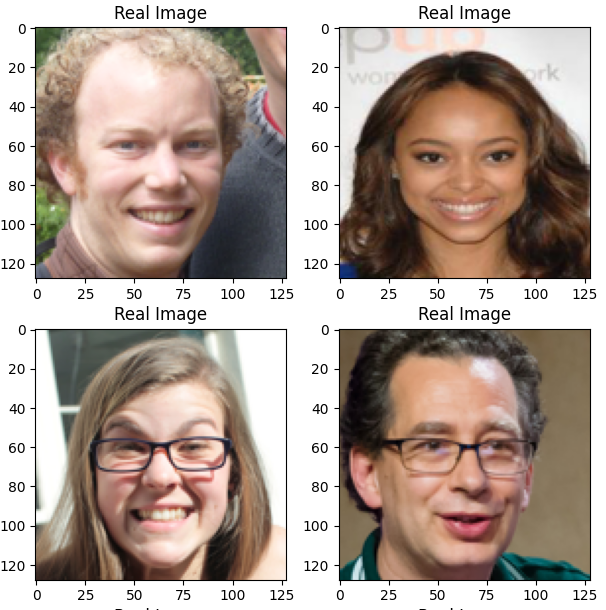
\includegraphics[width=0.95\linewidth]{./img/real sample.png}
				\caption{Real Images}
		\end{minipage}
		\hfill
		\begin{minipage}{0.45\textwidth}
				\centering
				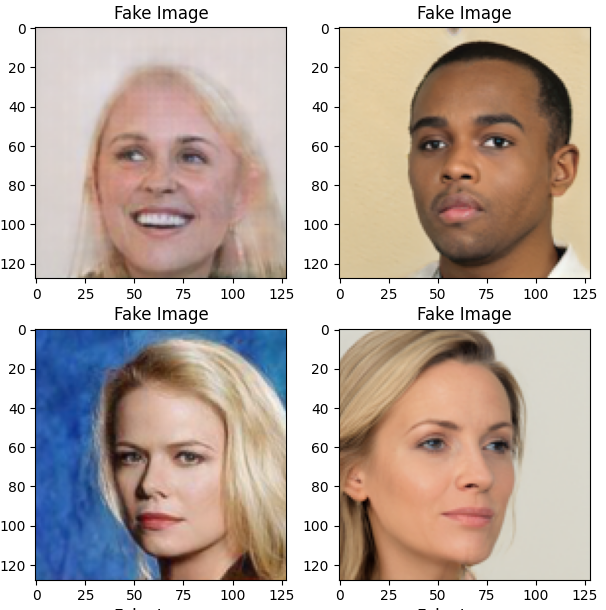
\includegraphics[width=0.95\linewidth]{./img/fake sample.png}
				\caption{Fake Images}
		\end{minipage}
	\end{figure}

	\section{Data Preprocessing}
	\subsection{Data Augmentation}
		To balance our dataset, we augmented our images to achieve a total of 25000 images for each category. For the 5000 fake images, we applied four different transformations, resulting in 20000 augmented fake images. For the real images, we randomly selected and transformed 3750 images, generating 15000 augmented real images. Various transformations, such as rotation, compression, scaling, and mirroring, were implemented. A sample of each transformation is shown below:

	\begin{figure}[hbt!]
		\centering
		\begin{minipage}{0.45\textwidth}
				\centering
				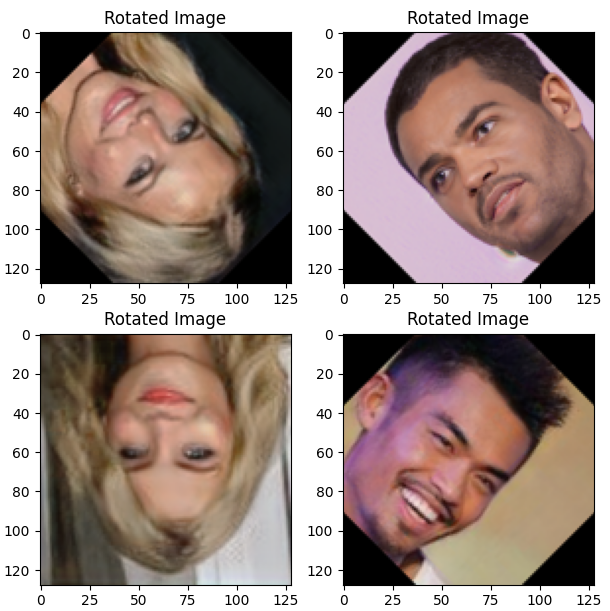
\includegraphics[width=0.95\linewidth]{./img/rotated.png}
				\caption{Rotated Images}
		\end{minipage}
		\hfill
		\begin{minipage}{0.45\textwidth}
				\centering
				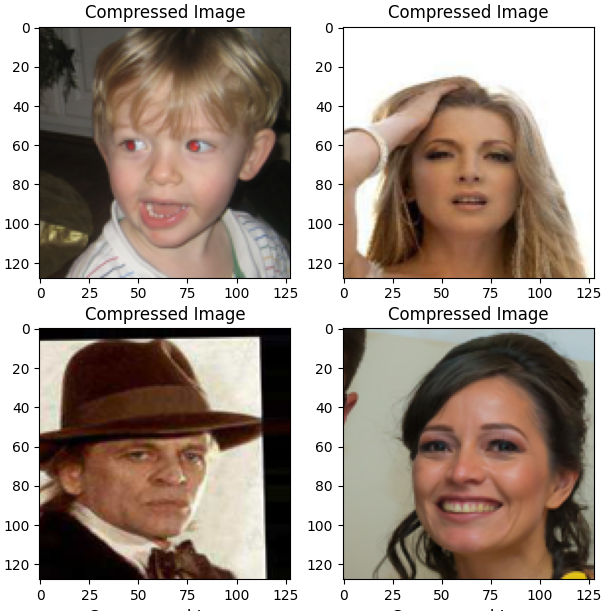
\includegraphics[width=0.95\linewidth]{./img/compressed.png}
				\caption{Compressed Images}
		\end{minipage}

		\vspace{0.5cm} % Add some vertical space between the two rows of images

		\begin{minipage}{0.45\textwidth}
				\centering
				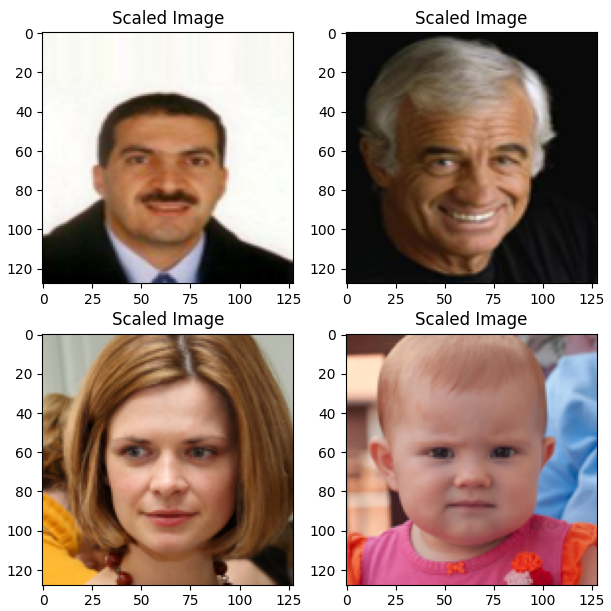
\includegraphics[width=0.95\linewidth]{./img/scaled.png}
				\caption{Scaled Image}
		\end{minipage}
		\hfill
		\begin{minipage}{0.45\textwidth}
				\centering
				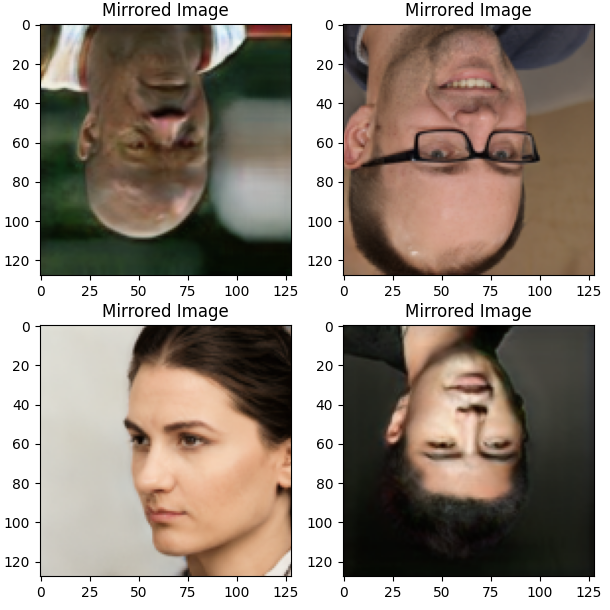
\includegraphics[width=0.95\linewidth]{./img/mirrored.png}
				\caption{Mirrored Images}
		\end{minipage}
	\end{figure}

	\subsection{Data Normalization}
	First, we computed the mean and standard deviation of the entire dataset, which consists of both the original dataset and the augmented dataset. The normalization process was then applied using the following formula:
	\begin{equation}
	x = \frac{x - \mu}{\sigma}
	\end{equation}
	where \(x\) represents the pixel values of each image pixel.
	
	This approach standardizes the features to have a mean of 0 and a standard deviation of 1. This standardization is crucial because certain machine learning algorithms are sensitive to the scale of the input features.

	\subsection{Data Splitting}
	We partitioned our dataset into a training set, comprising 80\% of the dataset, and a validation set, consisting of 20\% of the dataset. This division ensures that the model has an ample amount of data for learning, while also offering a subset of the data to assess the model's performance.

	\section{Setting Parameters}
	\begin{itemize}
		\item \textbf{Number of epochs : 50} \\
			The number of epochs refers to the number of times the complete training dataset is passed through the network during the training process. Each epoch consists of one forward pass (input to output) and one backward pass (error calculation and weight updates) for all the training samples.
		\item \textbf{Loss function : Cross-Entropy} \\
			Loss function is a method of evaluating how well your algorithm models your dataset. Cross-entropy loss measures the difference between a deep learning classification model's discovered and predicted probability distributions.

			The cross-entropy between two probability distributions, such as q from p, can be stated formally as
			
			\begin{equation}
				H(p, q) = -\sum_{x \in \mathcal{X}} p(x) \log q(x)
			\end{equation}

			Where
			\begin{itemize}
				\item H is the cross-entropy function
				\item p may be the target distribution
				\item q is the approximation of the target distribution.
			\end{itemize} 

		\item \textbf{Learning rate : 0.001} \\
			The learning rate is a hyperparameter that determines the step size at which an optimization algorithm.
		\item \textbf{Optimizer : Adam} \\
			An optimizer  is an algorithm used to update the parameters (weights and biases) of a model during training in order to minimize the loss function. 
			Adam (short for Adaptive Moment Estimation) is a popular optimization algorithm known for its robustness, efficiency, and ease of use. It often converges faster and performs better than traditional optimization algorithms.
			It adapts the learning rate for each parameter individually based on the past gradients and squared gradients making it well suited for training models.
	\end{itemize}

	\section{Model Training}
		We tested various customs models as well as pre-trained models like VGG16\_bn, ResNet50, ResNet101, and many more. During this process, We came to a conclusion that ResNet9 was performing much better than other models. So, We are using ResNet9 architecture for further training and implementation process.
		
		The model begins with an input layer configured to accept images with dimensions of 128x128 pixels and three color channels (RGB). Following this, the first convolutional layer is applied, utilizing 64 filters of size 3x3. Each filter convolves across the input image, extracting various features such as edges and textures. Batch normalization is then performed to normalize the activations of the convolutional layer, enhancing training stability. Subsequently, a rectified linear unit (ReLU) activation function is applied, introducing non-linearity to the network by replacing negative values with zeros.

		Moving forward, the second convolutional layer processes the output of the previous layer, applying 128 filters of size 3x3. Again, batch normalization and ReLU activation follow suit. Additionally, a max-pooling layer with a 2x2 window and a stride of 2 downsamples the feature maps, reducing spatial dimensions and computational complexity.

		Next, a residual block, inspired by the ResNet architecture, is introduced. This block comprises two convolutional layers, each followed by batch normalization and ReLU activation. The output of these layers is added to the output of the second convolutional layer, fostering better gradient flow during training and mitigating the vanishing gradient problem.

		Continuing, convolutional layer 3 is applied, employing 256 filters of size 3x3. Batch normalization and ReLU activation are again utilized for feature map normalization and non-linearity introduction, respectively. Another max-pooling layer further reduces spatial dimensions.

		Subsequently, convolutional layer 4 is employed, employing 512 filters of size 3x3. Similar to prior layers, batch normalization and ReLU activation are applied. Following this, another residual block, akin to ResNet architecture, is employed, aiding in feature extraction and gradient flow enhancement.

		Finally, a max-pooling layer with a 4x4 window reduces the spatial dimensions further. The resultant feature maps are then flattened into a 1D vector, which undergoes dropout regularization with a rate of 0.2, randomly deactivating 20\% of neurons during training to prevent overfitting. Lastly, a fully connected layer with two units, likely indicative of binary classification, applies a softmax activation function to generate class probabilities.
	\newpage
	\begin{figure}[hbt!]
		\center{
			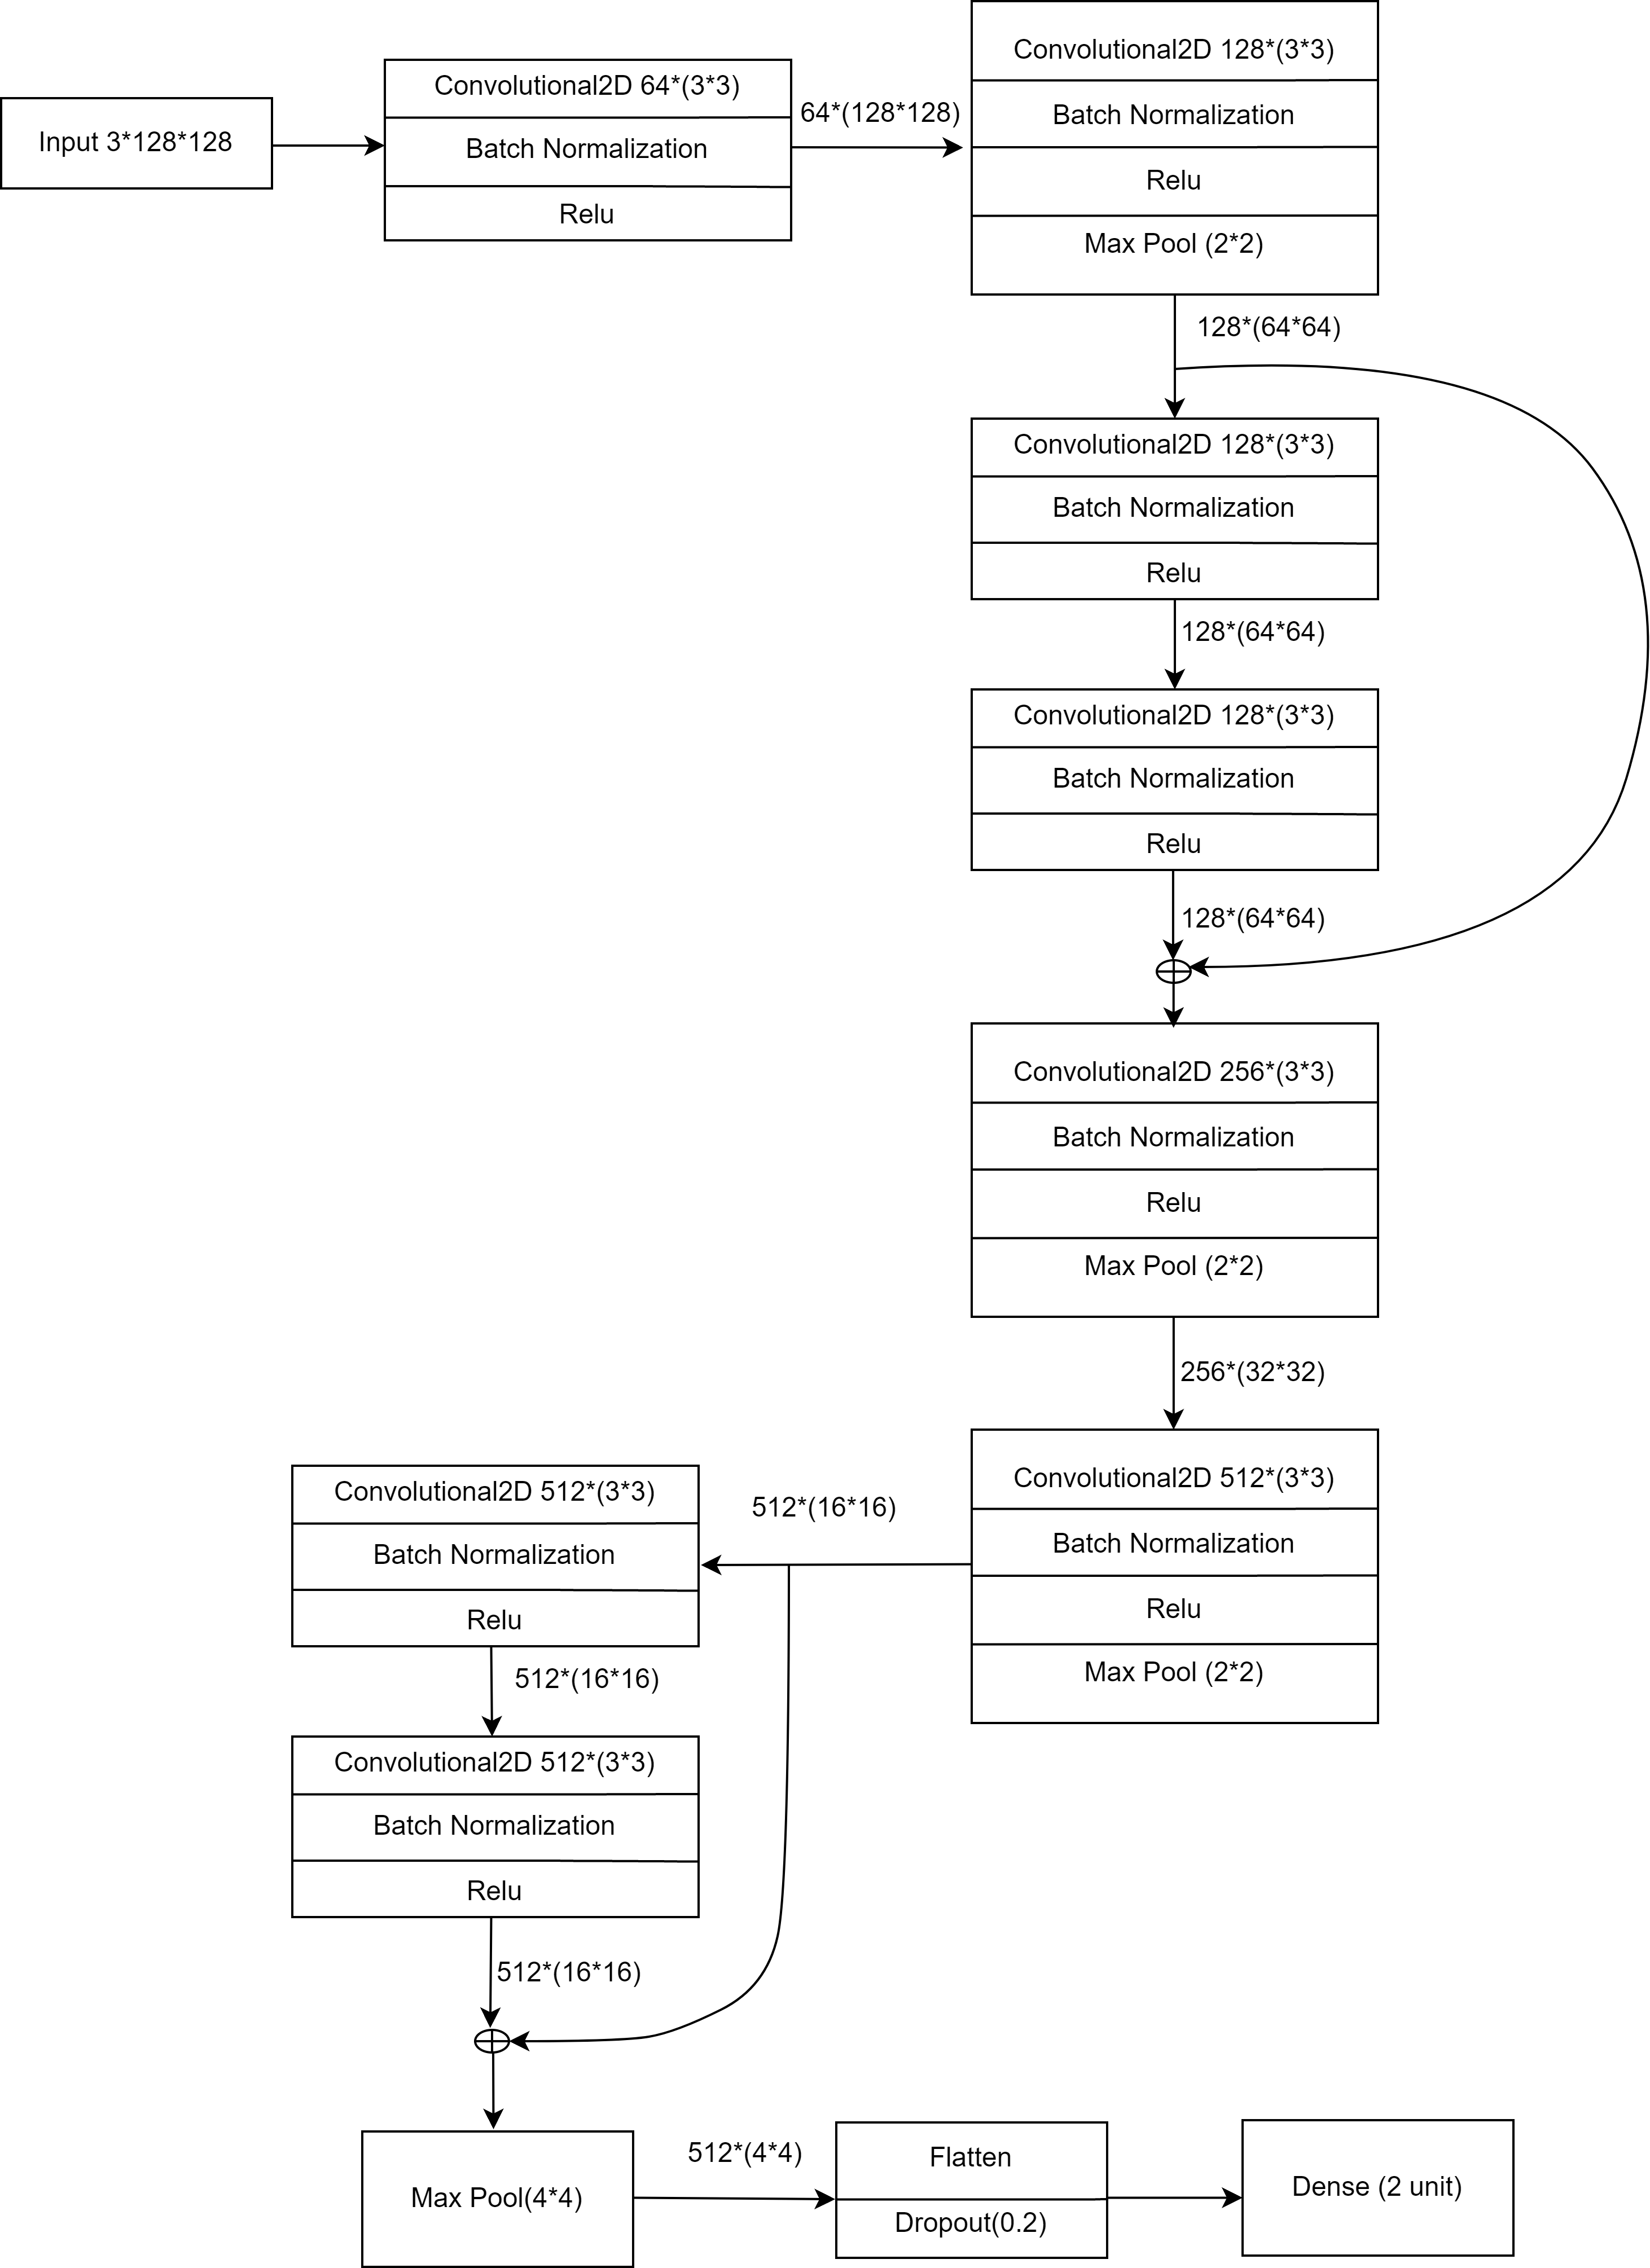
\includegraphics[width=0.68\textheight]{./img/layers.png}
			\caption{Architecture of ResNet9 Model}
		}
	\end{figure}

	\section{Model Evaluation}
	\begin{figure}[hbt!]
		\center{
			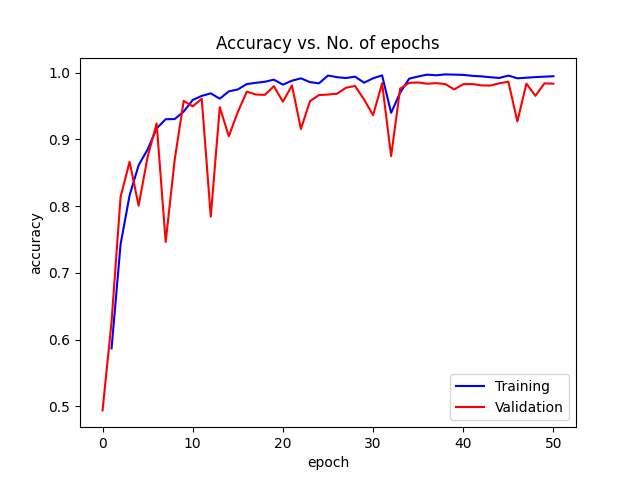
\includegraphics[width=0.8\textwidth]{./img/resnet9accuracy.png}
			\caption{Accuracy vs. No. of epochs }
		}
	\end{figure}
	\begin{figure}[hbt!]
		\center{
			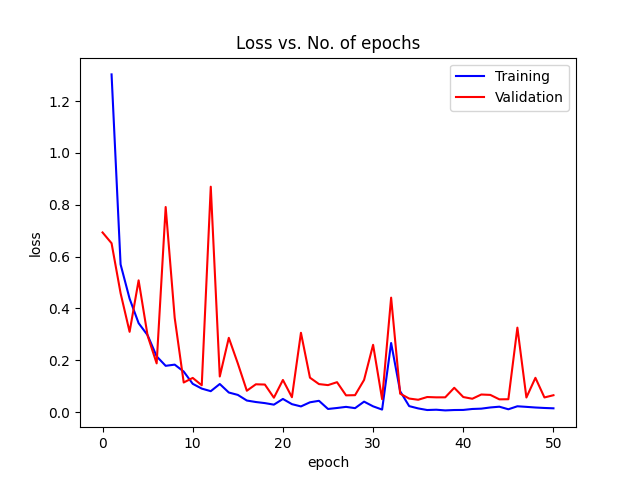
\includegraphics[width=0.8\textwidth]{./img/resnet9losses.png}
			\caption{Loss vs. No. of epochs}
		}
	\end{figure}

	\subsection*{Testing Results}
	We used the test dataset given on the DeepFake Detection Challenge\cite{jimaging8100263} to test our models performance.
	Testing dataset consist of 5000 fake images and 2000 real images.
	\vspace{1pt}
	\begin{figure}[hbt!]
		\center{
			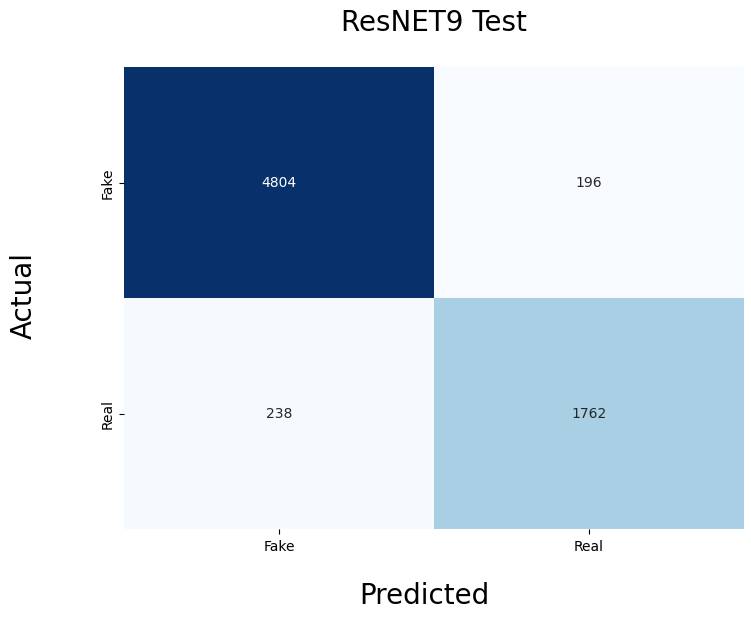
\includegraphics[width=1\textwidth]{./img/confusion_matrix.png}
			\caption{Confusion Matrix}
		}
	\end{figure}

	% \newpage
	\begin{enumerate}
		\item Accuracy
		\begin{equation}
				\text{Accuracy} = \frac{\text{TP} + \text{TN}}{\text{TP} + \text{TN} + \text{FP} + \text{FN}}
		\end{equation}
		\item Precision
		\begin{equation}
			% \begin{flalign}
				\text{Precision} = \frac{\text{TP}}{\text{TP} + \text{FP}}
			% \end{flalign}
		\end{equation}
		\item Recall
		\begin{equation}
			\text{Recall} = \frac{\text{TP}}{\text{TP} + \text{FN}}
		\end{equation}
		\item F1 Score
		\begin{equation}
			\text{F1 Score} = 2 \times \frac{\text{Precision} \times \text{Recall}}{\text{Precision} + \text{Recall}}
		\end{equation}

		where
		TP = True Positive,
		TN = True Negative,
		FP = False Positive,
		FN = False Negative
		\item Reciever Operating Characteristic (ROC) Curve
			\begin{figure}[hbt!]
				\center{
					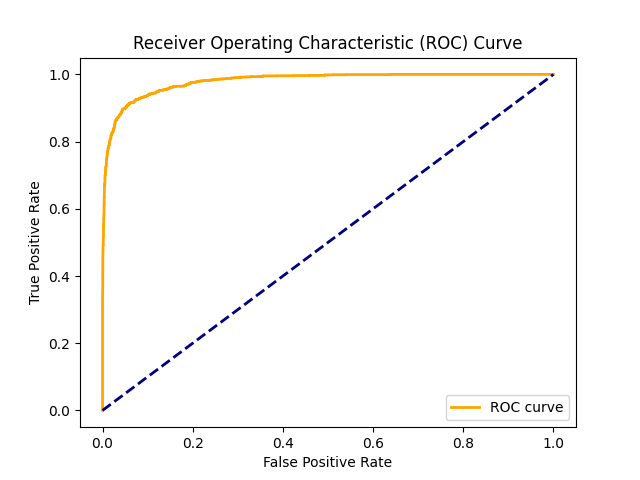
\includegraphics[width=1\textwidth]{./img/ROC.png}
					\caption{Reciever Operating Characteristic (ROC) Curve}
				}
			\end{figure}

			\textbf{Area Under ROC Curve = 0.9796}

\begin{table}[h!]
		\centering
		\begin{tabular}{lccccc}
		\multicolumn{6}{c}{\textbf{}} \\ 
		\multicolumn{6}{c}{\textbf{}} \\ 
		\textbf{} & \textbf{Accuracy} & \textbf{Precision} & \textbf{Recall} & \textbf{F1-score} & \textbf{Support} \\
		\textbf{Fake}  & 96.08\% & 0.952 & 0.960 & 0.955 & 5000 \\
		\textbf{Real} & 88.10\%  & 0.899 & 0.881 & 0.889 & 2000 \\
		\textbf{Macro Avg} & 92.09\% & 0.925 & 0.920 & 0.922 & 7000 \\
		\textbf{Weighted Avg} & 93.80\% & 0.936 & 0.938 & 0.937 &7000 \\ 
		\multicolumn{6}{c}{\textbf{}} \\
		\multicolumn{6}{c}{\textbf{}} \\
		\end{tabular}
		\caption{Performance Table}
		\end{table}
\end{enumerate}

\newpage
\section{User Interface}

\begin{figure}[hbt!]
	\center{
		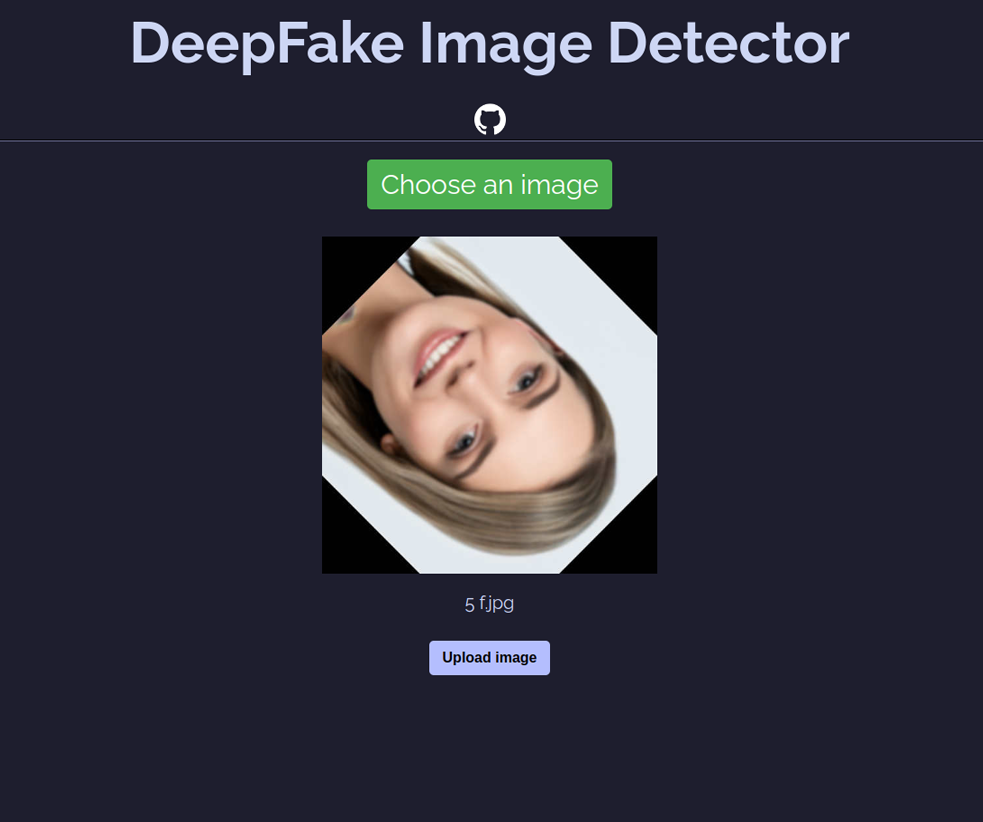
\includegraphics[width=0.66\textwidth]{./img/UI1.png}
		\caption{Demonstration of model detecting real image}
	}
\end{figure}
\begin{figure}[hbt!]
	\center{
		
\includegraphics[width=0.66\textwidth]{./img/UI2.jpg}
		\caption{Demonstration of model detecting fake image}
	}
\end{figure}
\end{document}